
\iffalse
\begin{figure}
    \centering
    \includegraphics[width=12cm]{../figures/blip_bbh_runs_two_panel_comparison.pdf}
    \caption{Glitch panel comparison}
    \label{fig:qscan_null}
\end{figure}
\fi
While the third-generation detectors are anticipated to push the accuracy and precision of our measurements to unprecedented levels, they will also be subject to new kinds of challenges compared to the current generation detectors. Here, I specifically compare the impact of glitches on GW signals detected by LIGO-Virgo interferometers and by 3G interferometers.
\begin{table}[h!]
    \centering
    \renewcommand{\arraystretch}{1.2}
    \begin{tabular}{p{0.45\textwidth}|p{0.45\textwidth}}
    \toprule
    \textbf{LIGO-Virgo interferometers} & \textbf{Third-generation interferometers} \\
    \midrule
    \begin{enumerate}[leftmargin=*, label=\arabic*.]
        \item Detection rate of $\mathcal{O}(1)$ signal per week
        \item A GW signal is in-band for $\mathcal{O}(1)$ second to $\mathcal{O}(1)$ minute. Therefore, nearly every segment of data contains only noise. 
        \item Glitch rate of $\mathcal{O}(1)$ per minute across three observation runs. 
        \item \textit{Almost} all glitches occur in isolation due to a smaller in-band duration and smaller detection rate of GW signals. 
        \item Almost all glitches can be vetoed (excluded from the analyses) without incurring a significant loss of GW signals. 
    \end{enumerate}
    &
    \begin{enumerate}[leftmargin=*, label=\arabic*.]
        \item Detection rate of $\mathcal{O}(1)$ signal per minute
        \item A GW signal is in-band for $\mathcal{O}(1)$ minute to $\mathcal{O}(1)$ hour. Therefore, nearly every segment of data is expected to contain a signal. 
        \item Glitch rate is unknown. Let's assume the same as LIGO-Virgo interferometers.
        \item \textit{Almost} all glitches will overlap with a GW signal due to a larger in-band duration and larger detection rate. 
        \item Very few glitches may be vetoed without losing GW signals. 
    \end{enumerate}
    \\
    \bottomrule
    \end{tabular}
    \caption{Impact of glitches on the LIGO-Virgo signals in comparison to the anticipated 3G signals.}
    \label{tab:glitch_diff}
\end{table}

When occurring in the vicinity of a GW signal, glitches (or transient noises) can corrupt the signal. Such signal-overlapping glitches must be carefully removed before analysing the signal. From the 90 confident events detected across three observation runs by LIGO-Virgo interferometers, about 20 were contaminated by glitches and required some form of glitch mitigation~\cite{KAGRA:2021vkt}. This number will continue to increase as the interferometers collect more data. A detailed study on how the physical interpretation of a GW signal may vary, depending on how a glitch in its proximity is removed, was conducted in the context of GW191109~\cite{Udall:2024ovp}. Specifically, it was argued that the interpretation of the spins of black holes may be affected. 

While glitch mitigation is an active area of research for current generation detectors, it is yet to receive similar attention in the context of 3G detectors. In Table~\ref{tab:glitch_diff}, we compare the problem posed by glitches for the LIGO-Virgo and the 3G interferometers. Glitches could be a major bottleneck in transitioning to the precision science era. In this chapter, we introduce the \texttt{nijntje} -- a null stream inspired noise transient elimination framework that is inexpensive, accurate, and scalable against the increasing computational cost of data analysis in the 3G-era. Through \texttt{nijntje}, we demonstrate a clear edge that the null stream, inherent in the triangular configuration of the Einstein Telescope, provides for the precision science era. 


\section{The null stream}
By definition, the null stream is a linear combination of strain data from a network of GW detectors such that the signal (if present in the strain) cancels out. For the triangular configuration of the Einstein Telescope (\ETT), the null stream can be constructed by summing the strain data from three detectors. Let us denote the data from $i^{\mathrm{th}}$ detector by $\vec{d}_i$,
\begin{equation}
 \vec{d}_i = F_{+, i} \vec{h}_+ + F_{\times, i} \vec{h}_{\times},
\end{equation}
where $i$ varies from 1 to 3, $F_{+, i}$ and $F_{\times, i}$ are the antenna pattern functions of $i$th interferometer. The notations $h_+$ and $h_{\times}$ represent the GW polarisations, defined in chapter~\ref{ch:gws}. The null stream is then constructed by;
\begin{equation}
    \label{eq:null-stream-eq}
 \vec{d}_{\mathrm{null}} = \frac{1}{\sqrt{3}}\sum_{i = 1}^{3}\vec{d}_i,
\end{equation}
where the prefactor of $1/\sqrt{3}$ ensures that the noise’s power spectral density of the null stream equals the average of those of the individual detectors. 

\begin{figure}
    \centering
    \includegraphics[width=\textwidth]{../figures/null_stream_antenna_pattern.pdf}
    \caption{Illustration of how the null stream of \ETT~comes about. Projection of plus (left) and cross (right) antenna pattern functions along the right ascension (RA) coordinate. Blue, red, and green lines show the antenna pattern functions of ET$_1$, ET$_2$, and ET$_3$, respectively. The black line, which is equal to zero for all values of RA, is obtained by summing the three. For simplicity, I only shown the projection along RA. The sum of the three is zero at all sky locations. This feature gives rise to an inherent null stream in the triangular configuration of ET.}
    \label{fig:sum_patterns}
\end{figure}

The null stream is a geometric feature of the triangle configuration of ET. It comes about from the fact that the sum of antenna pattern functions is individually zero \asam{Somewhere maybe the expressions for F+ and Fx; or you could put it in chapter 1 just after Eqn (1.33) and refer to it here as well.}, i.e.,
\begin{equation}
    \label{eq:sum_pattern}
    \sum_{i=1}^3 F_{+, i} = 0 ~ ~ \mathrm{and} ~ ~ \sum_{i=1}^3 F_{\times, i} = 0.
\end{equation}
We note that individual antenna pattern functions do vary over the whole sky (see Figure~\ref{fig:antenna_pattern} in chapter~\ref{ch:gws}). But the equalities presented in Eq.~\eqref{eq:sum_pattern} hold for the whole sky. As an illustration, we show the projection of antenna pattern functions along the right ascension (RA) coordinate in Figure~\ref{fig:sum_patterns}.

\section{\texttt{nijntje}: null-stream inspired noise transient elimination framework}
\label{sec:framework}
The null stream of the triangular ET enables a novel framework to remove signal-overlapping glitches. For brevity, we refer to it as \texttt{nijntje} -- null-stream inspired noise transient elimination -- framework. Figure~\ref{fig:nijntje_chart} shows the workflow of the \texttt{nijntje} framework. In this section, we explain the setup of our simulations and the operations within the \texttt{nijntje} framework.
\begin{figure}
    \centering
    \includegraphics[width=16cm]{../figures/assemble_nijntje.pdf}
    \caption{The blue box outlines the workflow of \texttt{nijntje} framework. \textit{Step 1}: Construct the null stream by summing the strain data from three interferometers. \textit{Step 2}: Using the null stream data and an RJMCMC method, perform an unmodelled reconstruction of the glitch time series. \textit{Step 3}: Subtract the glitch time series from $\mathrm{ET}_1$ data to obtain the \textit{cleaned} data. \textit{Step 4} (Optional): Perform parameter estimation of the GW signal using the cleaned data from $\mathrm{ET}_1$, and the existing data from $\mathrm{ET}_2$ and $\mathrm{ET}_3$ to verify the accuracy of glitch mitigation.}
    \label{fig:nijntje_chart}
\end{figure}
\subsubsection{Setup of the simulation}
We consider a typical scenario where a glitch overlaps with a GW signal. While the glitches exhibit a range of morphologies, here we choose a morphology that is ubiquitous in the data, i.e. the blips~\cite{Cabero:2019orq}. For the sake of the example, we assume that the only interferometer encounters the glitch. The rest of the two interferometers of the triangle contain a GW signal in Gaussian noise. The GW source is placed at a redshift of 2, where the merger rate distribution of BBH peaks, making it a typical source. The source frame masses of the two black holes are $38\,M_\odot$ and $33\,M_\odot$. We use the IMRPhenomD waveform model for our analysis. These configuration choices results in a GW signal with a network signal-to-noise ratio (SNR) of 83 divided equally among three interferometers. The starting frequency of our analysis is 20 Hz, the sampling frequency is 2048 Hz, and we use ET-D power spectral density (PSD) to simulate Gaussian noise. The ET-D PSD is currently the best prediction for what the noise PSD of ET may look like~\cite{Hild:2010id}. Each arm of the triangle is 10km long. We inject a blip glitch in the ET$_1$ interferometer that overlaps with the GW signal. We ensure that the SNR of the glitch is similar to the SNR of the GW signal in ET$_1$, i.e. $83/\sqrt{3} \sim 47$. Thanks to recent developments in machine learning based methods, it is now possible to simulate glitches.  
For example, the \texttt{gengli} codebase can generate blip glitches akin to the ones observed during the second observing run of Advanced LIGO and Virgo~\cite{Lopez:2022lkd, Lopez:2022dho}. An illustration of this setup is shown in the top panel of Figure~\ref{fig:nijntje_chart}. In our setup, the glitch is only in ET$_1$ interferometer, the rest of the two interferometers contain the GW signals in Gaussian noise.

\subsubsection{Executing the steps of \texttt{nijntje} framwork}
Following the steps outlined in Figure~\ref{fig:nijntje_chart}, we formulate the null stream in step 1. By construction, the null stream does not contain any signal. It only contains the glitch and the sum of Gaussian noise from three interferometers. To subtract the glitch, we first want to obtain the corresponding time series. We do this using the unmodelled reconstruction method described in chapter \ref{ch:bayeswave}. Indeed, we do not need to be concerned about the possible leakage from the GW signal while performing the glitch reconstruction using the null stream. 

In step 2, we reconstruct the glitch from the null stream. Specifically, we obtain the time series corresponding to the median parameters of the posterior samples. In step 3, we subtract it from the ET$_1$ interferometer data, making sure that it is scaled by a factor of $\sqrt{3}$ and the glitch onsets are aligned. This completes our step 3, and we finally \textit{cleaned} the glitch from ET$_1$. 

Next, to verify that our glitch mitigation is accurate, i.e., we have not removed part of the signal or we have not left behind a part of the glitch, we perform modelled reconstruction (also known as parameter estimation) on the GW signal, as described in chapter~\ref{ch:gwpe}. We can compare the parameter measurements obtained by analysing the cleaned data with the one obtained from the data when we do not introduce any glitch. The latter serves as the benchmark for our comparison. Indeed, the parameter estimation step can be used to test the quality of glitch mitigation only in a simulated setting. In reality, we do not have a benchmark for comparison. 

\section{Glitch mitigation in the absence of \texttt{nijntje} framework}
The framework \texttt{nijntje} is unique to the triangular geometry of the ET (\ETT). To compare \ETT~with an alternate configuration, we consider a network of two, distant L-shaped interferometers (referred to as ET-2L) located in Sardinia and the EMR region. In the absence of the \texttt{nijntje} framework, we perform a joint reconstruction of the GW signal and the glitch using the data from both interferometers. The joint modelling is prone to leakage, i.e, part of the glitch could be mismodelled as part of the signal and vice versa. Therefore, as introduced in Chatziioannou \textit{et al.}~\cite{Chatziioannou:2021ezd}, instead of modelling the GW signal itself with sine-Gaussian wavelets, a realistic signal model is employed with the expectation of reducing the mismodelling.

The setup of the simulation for the ET-2L network remains similar to the one described in section~\ref{sec:framework}. The GW signal parameters and the glitch morphology are the same as \ETT, leading to a GW network SNR of 124, with the Sardinia and EMR interferometers contributing SNRs of 90 and 85, respectively. The arm length of each interferometer is 15 km, and the power spectral density (ET-D) is scaled accordingly, resulting in a higher GW signal SNR compared to \ETT. The glitch is introduced in the Sardinia interferometer, whose SNR matches the glitch SNR in ${\rm ET}_1$. For this setup, we perform a glitch mitigation using the BayesWave codebase -- a routinely used tool to perform joint modelling of the GW signal and glitch coherently across the detector network~\cite{Cornish:2014kda, Cornish:2020dwh, Chatziioannou:2021ezd, Hourihane:2022doe}. To reiterate, the GW signal here is modelled using the signal model, i.e. the IMRPhenomD model, and the glitch is modelled using wavelets. 

One can model both the signal and the glitch using wavelets. This approach does not require prior knowledge of the GW signal model and, therefore, may seem ideal. However, this approach increases the amount of mismodelling and is hence not preferred~\cite{Chatziioannou:2021ezd}. 

\begin{figure}[h]
    \centering
    \includegraphics[width=.4\textwidth]{../figures/thesis_et2l_delta_glitch_overlap_glitch_master.pdf}\hspace{.5cm}
    \includegraphics[width=.4\textwidth]{../figures/thesis_newsnr_mismatch_comparison.pdf}
    \caption{Green (red) indicates the glitch reconstructed using \ETT~null stream (ET-2L) for the $\Delta t = 0$ case. Grey shows the strain, and black shows the simulated glitch. The null stream helps avoid glitch mismodeling, resulting in much closer agreement with the simulated glitch.}
    \label{fig:glitch_overlap}
\end{figure}

\section{Results of source parameter measurement: Triangle and 2L comparison}

For each configuration, \ETT~and 2L, we consider 9 different scenarios. All settings are kept identical across these scenarios except the time interval between the GW merger and glitch onset. For \ETT, we perform glitch mitigation using \texttt{nijntje} to obtain the cleaned data. For ET-2L, in absence of the \texttt{nijntje} framework, we perform glitch mitigation by doing joint signal plus glitch modelling. After the glitch is removed, we perform parameter estimation to quantify the accuracy of glitch mitigation. If the glitch mitigation is precise, the measurement should be similar to a scenario where a glitch is not introduced to the data. 

Before we present the parameter estimation results, we showcase the results of glitch mitigation, i.e., how close the reconstructed glitch is to the true glitch. This serves as a precursor to the parameter estimation results since accurate glitch mitigation leads to accurate parameter measurement of GW. A visualisation of the glitch reconstruction is presented in Figure~\ref{fig:glitch_overlap}. The ET triangle configuration, due to the null stream, achieves a more accurate glitch reconstruction by avoiding mismodeling from the GW signal. In contrast, for the ET-2L configuration, inevitably, some additional features from the signal are incurred. 

\begin{figure}[h]
    \centering
    \includegraphics[width=\textwidth]{../figures/newsnr_fig_4.pdf}
    \caption{Measurement of detector-frame total mass $M_{\rm total}$, luminosity distance $D_{\rm L}$, 
 and sky localisation. Green (red) colour represents posterior distributions when the glitch is 
 removed using the \ETT~null stream (ET-2L). Blue colour shows the measurements when no glitch is 
 introduced, serving as a benchmark for comparison, and dashed black lines indicate the true values. 
 The green posteriors accurately recover the true parameter values and show high consistency 
 with the benchmark. Though the red posterior for the total mass $M_{\rm total}$ recovers the true value, it shows clear signs of bias and widening. In contrast, the measurements of luminosity distance and sky location are biased and miss the true values.}
    \label{fig:delta_zero}
\end{figure}


\iffalse
\begin{figure}
    \centering
    \includegraphics[width=10cm]{../figures/newsnr_mismatch_comparison.pdf}
    \caption{Mismatch}
    \label{fig:mismatch}
\end{figure}
\fi
\subsubsection{Glitch onset coinciding with the GW merger}

Next, we turn to the results of parameter estimation when the glitch onset precisely coincides with the GW merger. Figure~\ref{fig:delta_zero} presents a comparison of the posterior distributions of the GW signal parameters after the glitch is mitigated, for $\Delta t = 0$. For all parameters shown, glitch mitigation with null stream for \ETT~results in posteriors 
that demonstrate high consistency and closely align with the benchmark results, where ``benchmark'' refers to a scenario when no glitch is introduced to the data.

For the ET-2L configuration, though the total mass $M_{\rm total}$ posterior shows clear signs of widening, it recovers the true value. This can be attributed to the SNR 
in the glitch-free interferometer, enabling intrinsic parameter recovery. In contrast, posteriors for extrinsic parameters, 
namely luminosity distance and sky location, are inconsistent with the benchmark's posteriors and miss the true value. 

\begin{figure}[h]
    \centering
    \includegraphics[width=.45\textwidth]{../figures/newsnr_rank_10_single_block_percentile_parameters_short.pdf}
    \caption{A comparison of the credible level of the true parameter value relative to the posterior 
 distributions for various time intervals $\Delta t$ between glitch onset and GW merger. 
 Credible levels are in standard deviation units $\sigma$, following a standard normal distribution. The parameters considered are luminosity distance $D_{\rm L}$ and sky location $\Omega$. Green (red) markers denote credible levels for the \ETT~null stream (ET-2L) based measurements, and the blue lines provide credible levels in the absence of a 
 glitch as a benchmark (dotted for $\Omega$, dashed for $D_{\rm L}$). For the null stream-based approach, the credible levels closely align with the benchmark, indicating accurate measurements. The posteriors for ET-2L lead to wider credible levels and generally exclude the true value, except for the edge cases where the glitch is sufficiently distant in time from the GW merger.}
    \label{fig:trend}
\end{figure}

\subsubsection{Glitch onset away from the GW merger}

Finally, we turn to the scenarios when the glitch does not coincide with the merger. Figure~\ref{fig:trend} shows that the characteristics of extrinsic parameter recovery remain consistent across different $\Delta t$ values. A negative (positive) value of $\Delta t$ implies that the glitch onset falls before (after) the GW merger. We show the measurements of distance ($D_{\mathrm{L}}$) and sky localisation $(\Omega)$. The sky localisation contours are constructed from the right ascension and declination measurements. 

For all time intervals considered, the~\ETT~configuration yields measurements where the true distance and sky location lie within $3\sigma$ and closely align with the no-glitch benchmark. In contrast, with the ET-2L configuration, the resulting measurements are wider or generally exclude the true values, except when the glitch onset is 100 ms before or 20 ms after the merger. We infer that at those values of $\Delta t$, the glitch is far enough from the GW signal to cause any biases. 


\section{Outlook and future work}
The null stream provides us with an extra piece of information in the form of Eq.~\eqref{eq:null-stream-eq}. For the first time, we quantitatively show how this information can be used to address a pressing problem in GW related measurements. Further, in the table \ref{tab:nijntje_conclusion}, we summarise the comparison between the \ETT~and ET-2L~configuration in the context of glitch mitigation. 

\begin{table}[h!]
    \centering
    \renewcommand{\arraystretch}{1.2}
    \begin{tabular}{p{0.45\textwidth}|p{0.45\textwidth}}
    \toprule
 Glitch mitigation using ET-2L & Glitch mitigation using \ETT \\
    \midrule
    \begin{enumerate}[leftmargin=*, label=\arabic*.]
        \item Biases expected in the measurements. \textcolor{white}{Skip this line.}
        \item The signal model needs to be known \textit{a priori}. Biases expected to worsen if the signal model is not known or incorrect.
        \item Difficult to scale to meet the demands of 3G-era. Specifically, to analyse the long, loud, and overlapping signals of the 3G-era. $\mathcal{O}(10)$ hours per analysis. \textcolor{white}{Skip this line as well. Skip this line as well.}
        \item Biases worsen when two interferometers have unequal SNRs, i.e, the signal is in the blind spot of one L but bright spot of another.
    \end{enumerate}
    &
    \begin{enumerate}[leftmargin=*, label=\arabic*.]
        \item Quality of measurements is nearly identical to the scenario when glitches are not introduced.
        \item Does not require any prior knowledge of the signal model. \textcolor{white}{Skip this line. Skip this line. Skip this line.}
        \item Enables an inexpensive, accurate, and easily scalable framework \texttt{nijntje}. A ready-to-use tool to analyse the long, loud, and overlapping signals using \ETT. The framework can be scaled to $\mathcal{O}(1)$ second per analysis.
        \item Individual interferometer SNRs do not matter. Blind spots do not play a role.
    \end{enumerate}
    \\
    \bottomrule
    \end{tabular}
    \caption{Comparison \ETT~and ET-2L configuration in context of glitch mitigation}
    \label{tab:nijntje_conclusion}
\end{table}

\subsubsection{Implication on the science cases}

In the absence of the null stream, the sky location and luminosity distance measurements of the GW source are subject to significant biases due to mismodeling of glitches, even if the signal model is accurately known. Such biases could be harmful to science cases measuring cosmological parameters, in particular the ``dark siren'' method, which relies on three-dimensional volumetric matching between GW detections and galaxy catalogs~\cite{Schutz:1986gp, DelPozzo:2011vcw, Chen:2017rfc, LIGOScientific:2018gmd, Gray:2019ksv, LIGOScientific:2021aug, Palmese:2021mjm}; the null stream will be of help here. 

Similarly, ET is anticipated to reconstruct the merger rate distributions as a function of redshift. This is achieved by converting the GW distance measurements to a redshift using a cosmological model~\cite{Branchesi:2023mws}. This science case will benefit from the null stream.  

The ET is also expected to provide a unique opportunity to perform multimessenger astronomy. By producing early warning alerts, i.e. information about the sky-localisation of the GW signal before they merge, ET can help observe any electromagnetic emission associated with the GW merger, with the help of EM observatories~\cite{Cannon:2011vi, LIGOScientific:2017ync}. An incorrect or biased sky localisation due to glitches may hinder our ability to produce early warning alerts.

Searches for strong lensing of GW signals look for overlaps between the parameters of two GW signals~\cite{LIGOScientific:2023bwz}. The reconstruction of the lens galaxy also relies on accurate measurements of GW parameters, including distance and sky-localisation. Biases in these measurements due to glitches could be harmful to strong lensing searches and follow-up lens reconstruction~\cite{Poon:2024zxn, Wempe:2022zlk, Hannuksela:2020xor}. 

Searches for anomalous dispersion of gravitational waves due to violations of general relativity also require accurate distance measurements~\cite{LIGOScientific:2021sio}. Biases caused in the distance measurements due to glitches could be harmful here as well. Another science cases that require accurate distance measurements is the search for anomalous propagation of gravitational waves, discussed in more detail in chapter~\ref{ch:mod_prop}.

We note that in studies where information from multiple GW sources is combined, it will often be a relatively limited set of loudest signals that drive the combined result (tests of general relativity being a clear example \cite{LIGOScientific:2021sio}). If measurements on even a small fraction of these events are corrupted, it could adversely affect inference on the population as a whole. 

\subsubsection{Future work}
We plan to extend this work by including various kinds of signals and glitches in our analysis. Inspired by the seminal work of Dooney \textit{et al.}~\cite{Dooney:2025bfh}, the integration of a deep learning based noise mitigation tool into the \texttt{nijntje} framework is already underway. This feature will enable \texttt{nijntje} framework to run on GPUs, leading to a real-time glitch mitigation ($\mathcal{O}(1)$ second per glitch) and overall a sustainable approach for computation. 

We also plan to investigate the possibility of occurrence and mitigation of coincident glitches, i.e., glitches that appear in all interferometers of a network at the same time. We also plan to investigate the impact of Newtonian noise -- the models of which remain largely uncertain at the time of writing of this thesis. In addition, the null stream can be constructed when all three interferometers are online. We leave it to future work to include the duty cycle in our analyses. Note that, in the absence of a null stream, one can revert to performing joint signal and glitch mitigation for the triangular configuration. Indeed, the duty cycle will affect ET-2L as well. In the events when one of the two Ls is offline, the performance of glitch mitigation and GW parameter estimation is expected to worsen.	

The problem posed by glitches to the current and next-generation GW detectors is a pressing one. It could hinder our transition to the precision science era. The comparison presented in this chapter shows a clear edge that the null stream inherent in the triangular configuration has to offer over the alternate configuration. 

